\section{Proposed Services and Tools}
This section proposes new and better backend and frontend services that will enable the smooth operation of maintaining the website's infrastructure, development, and content. Each proposed service also includes the issue that they fix. Prices are in United States Dollars (USD), as these are the prices provided on each service's website.

\subsection{Sanity}
Sanity is a \textit{headless} CMS\@. Our current CMS, Wordpress, is not a headless CMS, because it also serves a frontend that shows the content from the CMS to readers (§3.1 fig.~\ref{fig:frame1}). A headless CMS gives more flexibility to designers and web developers who want granular control over the UI/UX of the frontend product; the way content is displayed and the content itself are decoupled entities.

\begin{figure}[H]
    \centering
    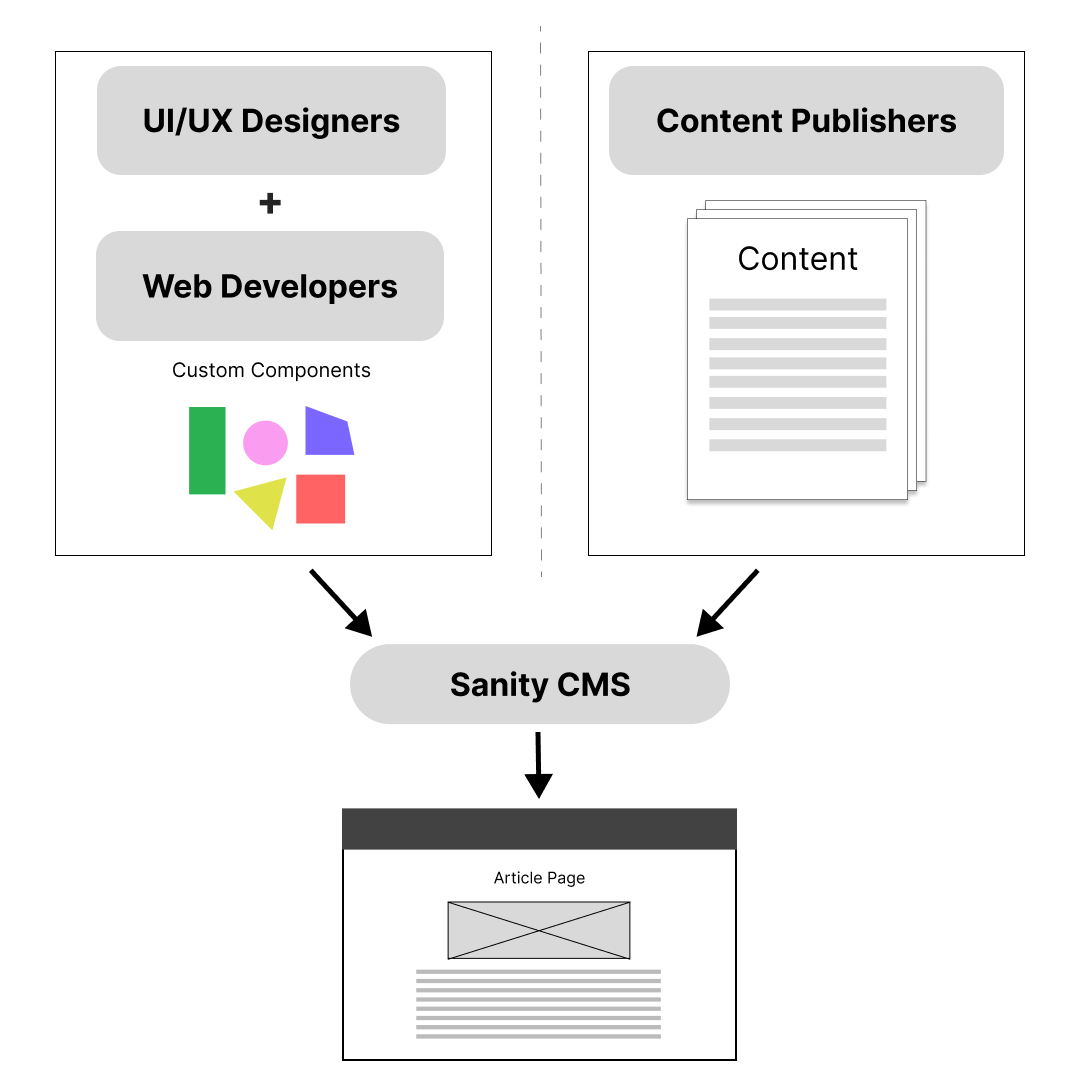
\includegraphics[scale=0.25]{diagrams/Sanity Diagram 1.png}
    \caption{Sanity combines components and content for the frontend.}
    \label{fig:sanity1}
\end{figure}

\subsubsection*{Features}
Since content and UI/UX design are separated, writers and publishers will not need to treat design as an afterthought. Sanity translates the results of the collaboration between web developers and UI/UX designers into a domain in which non-technical publishers are able to design a page, regardless of the page's content, to their liking. Designers create the design of UI/UX components, which are essentially pieces that come together to form the look and feel of the web page. They pass the design schemes to web developers to implement them into real code. Sanity consumes this component code and prepares it for writers and publishers to incorporate into their content on the frontend. Publishers can then combine both written content and custom components to create articles or web pages that are published on the frontend, without having to design or write a line of code. This approach can satisfy the customizability needs of the website to have a more coherent UI/UX design language, as well as future-proofing since components created now can be used well into the future.

\subsubsection*{Price}
\href{https://www.sanity.io/pricing}{Sanity's pricing} is transparent\footnote{https://www.sanity.io/pricing}. Many platforms gate functionality by price structure – higher priced tiers receive better functionality. Thankfully, nearly everything we need is provided in their first tier, the `Free Forever' plan.

Their pricing structure more-so delineates available usage quotas of different resources they provide in every tier. Similar to a phone plan, these quota limits describe how much data we are using per month to operate on their platform. I am most concerned with these five resources, in order of priority:

\begin{table}[H]
    \setlength{\tabcolsep}{10pt} % Default value: 6pt
    \renewcommand{\arraystretch}{1.5} % Default value: 1
    \begin{tabular}{ l l c }
        Assets & \$1 per 2 Gigabytes additional Assets per month\\
        CDN Requests & \$1 per 250,000 additional CDN Requests per month\\
        Documents & \$2.5 per 1,000 additional Documents per month\\
        Bandwidth & \$1 per 5 Gigabytes additional Bandwidth per month\\
        API Requests & \$1 per 25,000 additional API Requests per month\\
    \end{tabular}
\end{table}

An asset is any type of digital media. Assets on our website are images or audio. CDN Requests, Bandwidth, and API Requests are all related to frontend to backend communication, or values that quantify how much communication is happening. Documents is the number of data stored in the text database\footnote{Refer to §3 for a refresher on the infrastructure.}.

Below is a small table categorizing the quotas into two categories: Fluctuating and Fixed. The Fluctuating category is based on communication usage, like texting and call data on a phone plan: the more you text and call, the more money leaves your wallet. The Fixed category is based on storage usage, like Google Drive. It is called `Fixed' because it does not fluctuate as drastically as communication usage. The rate at which storage usage changes over time is significantly longer than communication usage based on a shorter time interval like those in the fluctuating category.

\begin{table}[H]
    \centering
    \setlength{\tabcolsep}{10pt} % Default value: 6pt
    \renewcommand{\arraystretch}{1.5} % Default value: 1
    \begin{tabular}{ l l }
        \textbf{Fluctuating} & \textbf{Fixed} \\
        CDN Requests & Assets \\
        Bandwidth & Documents \\
        API Requests & \\
    \end{tabular}
\end{table}

The Free Forever plan offers a free 5 gigabytes of asset storage. Every byte after 5 gigabytes will then be a charge on our account. Using 6 gigabytes (5 gigabytes + 1 extra gigabyte) means we will be charged \$1 extra for asset storage monthly. Using 7 gigabytes (5 gigabytes + 2 extra gigabytes) means a charge of \$2 to our account. Over time, storage use usually increases. This means that using the new website will incur additional asset storage fees. Since our asset storage will most likely be used to store images rather than bulkier media like video, this storage usage increase will be slow\footnote{On a more technical tangent, if images are uploaded in a lossy compression format like JPEG, and assuming that every picture is on average 5 megabytes, it would require 400 photos to use 2 gigabytes of storage. Even then, JPEG compression can reach sub-megabyte compression into kilobyte compression territory; if images were rather 600 kilobytes in size, it would require around 3300 images to use 2 gigabytes of storage. What a drastic decrease!}.

The Free Forever plan also offers free storage for 10,000 documents. A document can be imagined as a literal paper sheet with information on it; newspaper articles, acceptance letters, advertisements, and identification cards all fall under the term `document'. We can store 10,000 of these. The small catch is that revisions to a document count as an additional document. Therefore, revisions on the platform should be kept to a minimum to ensure maximum space optimization. This storage increase will follow the same financial trajectory as the asset storage: the more we store, the more the permanent cost, but the time to reach these costs is extremely slow.

Unless we hit an interstellar home run and become famous overnight, the amount of CDN Requests, Bandwidth, and API Requests should not breach the Free Forever plan's free quota thresholds. The only case when I suspect a breach would happen is when we are in the process of transitioning to the new website when we upload content to it in large batches, and even then, the fee charge will be minute given their prices of \$1.

In theory, if we were to keep our margins within the given usage limits of Sanity's Free Forever plan, we would spend absolutely no money. In practice, this is impossible, but the charges are meaningful, warranted, and reasonable given the size of our organization.

\subsection{Vercel}
Vercel provides website hosting, named \textit{Vercel Frontend Cloud}, for frontend projects. Vercel manages the nitty-gritty of hosting the frontend of a website, and lets its users concentrate on the website's design, development, and code, rather than being impeded by technicalities. Vercel is accessible because \href{https://vercel.com/docs}{their documentation}\footnote{https://vercel.com/docs} for developers and management alike is easily found online. It is robust because of their global content delivery network\footnote{https://vercel.com/features/infrastructure}. Finally, it is future-proof because many high-profile companies, such as Adobe, eBay, and The Washington Post, implement their services\footnote{https://vercel.com/customers}.

\subsubsection*{Price}
They have a very generous \href{https://vercel.com/pricing}{free tier plan}\footnote{https://vercel.com/pricing}. At this moment, we do not need the Pro Plan, which is \$20 a month, because the features are somewhat irrelevant to our needs. If an upgrade is ever needed in the future, I will notify those who may be of concern. Therefore, the total price to implement Vercel into the website infrastructure is \$0.

\subsection{Cloudflare}
Cloudflare services and maintains digital cloud infrastructure across the globe. Cloudflare has good qualities in the three trait categories. Cloudflare is accessible: the UI/UX is simple and clear. Access to different settings and functions is clearly labeled. In the event that something may be unclear, their \href{https://developers.cloudflare.com}{online documentation}\footnote{https://developers.cloudflare.com} and \href{https://blog.cloudflare.com/}{blog}\footnote{https://blog.cloudflare.com} is accessible and digestible. The services they provide are robust, dependable, and future-proof because a sizable majority of the internet flows through their worldwide data centers. Simply put, cloud security and internet infrastructure is their domain. Because of this, they provide backend service products we're particularly interested in: their registrar and image storage.

\subsubsection*{Domain Registrar}
In the technical community, using GoDaddy is a sin; any other domain registrar is better than GoDaddy. I chose Cloudflare's product, named \textit{Registrar}, because of its metric gathering and ease of use. Cloudflare is also one of several domain registrars that offer a \href{https://cloudflare.com/application-services/products/ssl/}{free certificate}\footnote{https://cloudflare.com/application-services/products/ssl/} for any domain on their platform, along with enhanced customizability for \href{https://developers.cloudflare.com/ssl/get-started}{certificate options and security}\footnote{https://developers.cloudflare.com/ssl/get-started}. Cloudflare's analytics and metrics aggregation is also top-tier.

\begin{figure}[h]
    \centering
    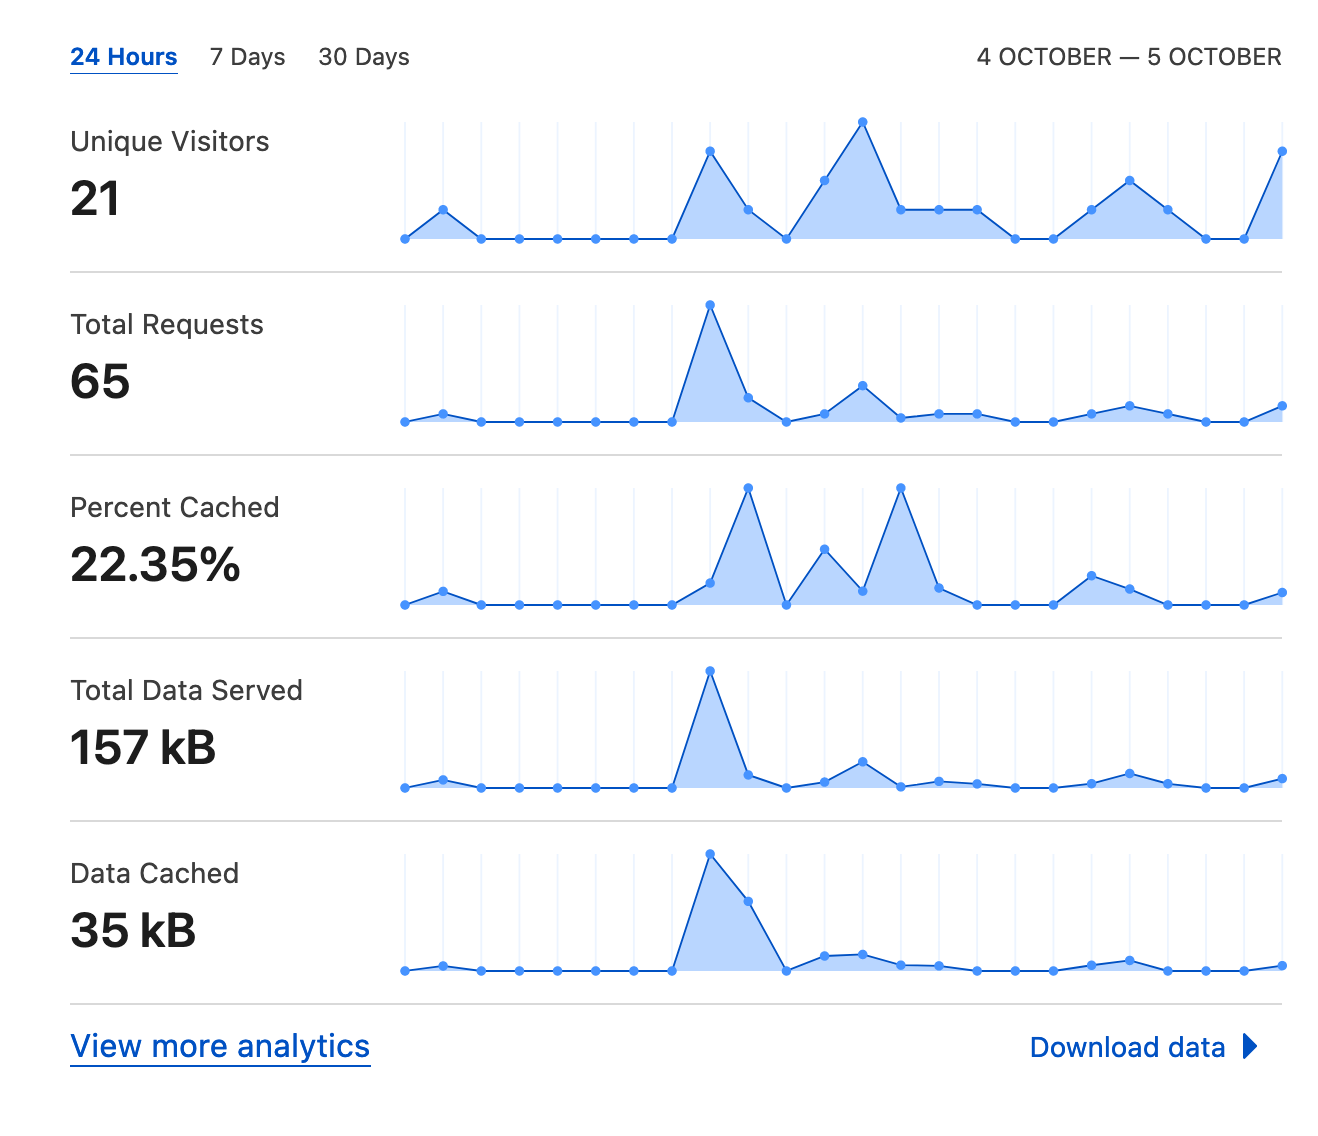
\includegraphics[scale=0.4]{pictures/CloudflareMetrics.png}
    \caption{A view of the Cloudflare Registrar domain metrics dashboard.}
    \label{fig:metrics}
\end{figure}

Please note that readers who view the website will be unaware of this registrar switch – visiting the OMS URL will still display the same website content before the switch. It does not affect the frontend.

\subsubsection*{Image Storage}
\href{https://www.cloudflare.com/developer-platform/cloudflare-images/}{\textit{Cloudflare Images}} is Cloudflare's image storage solution\footnote{https://www.cloudflare.com/developer-platform/cloudflare-images/}. Since the cPanel media database would no longer exist, Cloudflare is able to store and deliver any images we upload to Sanity. This service may or may not be used, depending on cost assessment of using Sanity's \textit{Content Lake}. However, this option exists as a backup, and their prices are affordable.

\subsubsection*{Price}
We are overpaying for our domain name at GoDaddy. They charge more than double that of Cloudflare's offering for our domain name.

At the time of this writing, Cloudflare's domain registrar sells domains with the \textit{com} TLD at a flat rate of \$9.77  a year\footnote{A Cloudflare account is required to access the domain pricing list. Since I have one, I was able to retrieve this price.}. Their image storage service starts at \$5  a month to store 100,000 images. Delivering 100,000 images costs \$1  extra for the monthly period. `Serving' an image means displaying it on our website. If we were to serve 99,999 images, we would not pay \$1. If we were to serve 500,000 images, we would have to pay \$5.

The total cost \textit{without} using Cloudflare Images is \$9.77 a year. This does not include local taxes. The total cost with Cloudflare Images is \$69.77 a year, since \$5 a month equates to \$60 for an entire year. This price does not take into account the fee for extra images served.
